\documentclass[]{article}
\usepackage{lmodern}
\usepackage{amssymb,amsmath}
\usepackage{ifxetex,ifluatex}
\usepackage{fixltx2e} % provides \textsubscript
\ifnum 0\ifxetex 1\fi\ifluatex 1\fi=0 % if pdftex
  \usepackage[T1]{fontenc}
  \usepackage[utf8]{inputenc}
\else % if luatex or xelatex
  \ifxetex
    \usepackage{mathspec}
    \usepackage{xltxtra,xunicode}
  \else
    \usepackage{fontspec}
  \fi
  \defaultfontfeatures{Mapping=tex-text,Scale=MatchLowercase}
  \newcommand{\euro}{€}
\fi
% use upquote if available, for straight quotes in verbatim environments
\IfFileExists{upquote.sty}{\usepackage{upquote}}{}
% use microtype if available
\IfFileExists{microtype.sty}{\usepackage{microtype}}{}
\usepackage[margin=1in]{geometry}
\usepackage{color}
\usepackage{fancyvrb}
\newcommand{\VerbBar}{|}
\newcommand{\VERB}{\Verb[commandchars=\\\{\}]}
\DefineVerbatimEnvironment{Highlighting}{Verbatim}{commandchars=\\\{\}}
% Add ',fontsize=\small' for more characters per line
\newenvironment{Shaded}{}{}
\newcommand{\KeywordTok}[1]{\textcolor[rgb]{0.00,0.44,0.13}{\textbf{{#1}}}}
\newcommand{\DataTypeTok}[1]{\textcolor[rgb]{0.56,0.13,0.00}{{#1}}}
\newcommand{\DecValTok}[1]{\textcolor[rgb]{0.25,0.63,0.44}{{#1}}}
\newcommand{\BaseNTok}[1]{\textcolor[rgb]{0.25,0.63,0.44}{{#1}}}
\newcommand{\FloatTok}[1]{\textcolor[rgb]{0.25,0.63,0.44}{{#1}}}
\newcommand{\ConstantTok}[1]{\textcolor[rgb]{0.53,0.00,0.00}{{#1}}}
\newcommand{\CharTok}[1]{\textcolor[rgb]{0.25,0.44,0.63}{{#1}}}
\newcommand{\SpecialCharTok}[1]{\textcolor[rgb]{0.25,0.44,0.63}{{#1}}}
\newcommand{\StringTok}[1]{\textcolor[rgb]{0.25,0.44,0.63}{{#1}}}
\newcommand{\VerbatimStringTok}[1]{\textcolor[rgb]{0.25,0.44,0.63}{{#1}}}
\newcommand{\SpecialStringTok}[1]{\textcolor[rgb]{0.73,0.40,0.53}{{#1}}}
\newcommand{\ImportTok}[1]{{#1}}
\newcommand{\CommentTok}[1]{\textcolor[rgb]{0.38,0.63,0.69}{\textit{{#1}}}}
\newcommand{\DocumentationTok}[1]{\textcolor[rgb]{0.73,0.13,0.13}{\textit{{#1}}}}
\newcommand{\AnnotationTok}[1]{\textcolor[rgb]{0.38,0.63,0.69}{\textbf{\textit{{#1}}}}}
\newcommand{\CommentVarTok}[1]{\textcolor[rgb]{0.38,0.63,0.69}{\textbf{\textit{{#1}}}}}
\newcommand{\OtherTok}[1]{\textcolor[rgb]{0.00,0.44,0.13}{{#1}}}
\newcommand{\FunctionTok}[1]{\textcolor[rgb]{0.02,0.16,0.49}{{#1}}}
\newcommand{\VariableTok}[1]{\textcolor[rgb]{0.10,0.09,0.49}{{#1}}}
\newcommand{\ControlFlowTok}[1]{\textcolor[rgb]{0.00,0.44,0.13}{\textbf{{#1}}}}
\newcommand{\OperatorTok}[1]{\textcolor[rgb]{0.40,0.40,0.40}{{#1}}}
\newcommand{\BuiltInTok}[1]{{#1}}
\newcommand{\ExtensionTok}[1]{{#1}}
\newcommand{\PreprocessorTok}[1]{\textcolor[rgb]{0.74,0.48,0.00}{{#1}}}
\newcommand{\AttributeTok}[1]{\textcolor[rgb]{0.49,0.56,0.16}{{#1}}}
\newcommand{\RegionMarkerTok}[1]{{#1}}
\newcommand{\InformationTok}[1]{\textcolor[rgb]{0.38,0.63,0.69}{\textbf{\textit{{#1}}}}}
\newcommand{\WarningTok}[1]{\textcolor[rgb]{0.38,0.63,0.69}{\textbf{\textit{{#1}}}}}
\newcommand{\AlertTok}[1]{\textcolor[rgb]{1.00,0.00,0.00}{\textbf{{#1}}}}
\newcommand{\ErrorTok}[1]{\textcolor[rgb]{1.00,0.00,0.00}{\textbf{{#1}}}}
\newcommand{\NormalTok}[1]{{#1}}
\usepackage{graphicx}
\makeatletter
\def\maxwidth{\ifdim\Gin@nat@width>\linewidth\linewidth\else\Gin@nat@width\fi}
\def\maxheight{\ifdim\Gin@nat@height>\textheight\textheight\else\Gin@nat@height\fi}
\makeatother
% Scale images if necessary, so that they will not overflow the page
% margins by default, and it is still possible to overwrite the defaults
% using explicit options in \includegraphics[width, height, ...]{}
\setkeys{Gin}{width=\maxwidth,height=\maxheight,keepaspectratio}
\ifxetex
  \usepackage[setpagesize=false, % page size defined by xetex
              unicode=false, % unicode breaks when used with xetex
              xetex]{hyperref}
\else
  \usepackage[unicode=true]{hyperref}
\fi
\hypersetup{breaklinks=true,
            bookmarks=true,
            pdfauthor={Justin Le},
            pdftitle={Fun With MonadPlus: The Success/Failure Monads},
            colorlinks=true,
            citecolor=blue,
            urlcolor=blue,
            linkcolor=magenta,
            pdfborder={0 0 0}}
\urlstyle{same}  % don't use monospace font for urls
% Make links footnotes instead of hotlinks:
\renewcommand{\href}[2]{#2\footnote{\url{#1}}}
\setlength{\parindent}{0pt}
\setlength{\parskip}{6pt plus 2pt minus 1pt}
\setlength{\emergencystretch}{3em}  % prevent overfull lines
\setcounter{secnumdepth}{0}

\title{Fun With MonadPlus: The Success/Failure Monads}
\author{Justin Le}

\begin{document}
\maketitle

\emph{Originally posted on \textbf{\href{http://home.jle0.com:4111/entry/ident/list-monad.html}{in
Code}}.}

Monads. Haskell's famous for them, but they are one of the most ill-understood concepts to the
public. They are mostly shrouded in mystery because of their association with how Haskell models
I/O. This reputation is undeserved. Monads don't have anything to do with I/O.

This series is a part of a global effort to deshroud the mystery behind monads and show that they
are fun! And exciting! And really just a way of chaining together functions that allow for new ways
of approaching puzzles.

At the end of it all, we are going to be solving the classic logic puzzle, as old as time itself,
using the List monad:

\begin{quote}
A farmer has a wolf, a goat, and a cabbage that he wishes to transport across a river.
Unfortunately, his only boat can carry one thing at a time. He can't leave the wolf alone with the
goat, or the wolf will eat the goat. He can't leave the goat alone with the cabbage, or the goat
will eat the cabbage. How can he properly transport his belongings to the other side one at a time,
without any disasters?
\end{quote}

Let us enter a brave new world!

\section{Monads, Reviewed}\label{monads-reviewed}

As a Haskell blogger, I'm not allowed to write any straight-up monad tutorials, but I don't need too
--- there are a wealth of great ones.
\href{http://adit.io/posts/2013-04-17-functors,_applicatives,_and_monads_in_pictures.html}{Adit
provides a great concise one}, and, if you want,
\href{http://www.haskell.org/haskellwiki/All_About_Monads}{a more in depth one} is on the
haskell.org wiki about using them in real life.

However, here is a short description of ``monadic style'', as it applies to what we are going to do
today.

Remember --- different monads do not actually have any non-superficial relationship to one another.
When we say monads, we just mean things that chain together functions ``inside'' wrappers,
containers, or contexts. In our case, containers.

\section{Maybe, maybe not}\label{maybe-maybe-not}

Let's look at the most obvious container -- a \texttt{Maybe\ a}. A \texttt{Maybe\ a} is a container
that can either be \texttt{Just\ a} (representing a succesful result \texttt{a}) or a
\texttt{Nothing} (representing a failed result).

\begin{verbatim}
###### Aside
\end{verbatim}

Hi! These asides are going to be for you readers that are unfamiliar with Haskell syntax. Feel free
to ignore them if you already feel comfortable.

Anyways, if you've ever done any object-oriented programming, you might be able to think of
\texttt{Maybe\ a} as an abstract/virtual superclass with templates/generics ---
\texttt{Maybe\textless{}a\textgreater{}}, kinda. And that superclass has two subclasses:
\texttt{Just\textless{}a\textgreater{}}, which has one public instance variable of type \texttt{a},
and \texttt{Nothing}, which contains no instance variables.

Often times you'll have functions that fail, and you want to chain them. The easiest way is that any
function that is chained onto a failed value will be skipped; a failure is the final result.

Consider the \texttt{halve} function, which returns \texttt{Just\ (x\ `div`\ 2)} on a succesful
halving, or \texttt{Nothing} on an unsuccesful halving:

\begin{Shaded}
\begin{Highlighting}[]
\OtherTok{halve ::} \DataTypeTok{Int} \OtherTok{->} \DataTypeTok{Maybe} \DataTypeTok{Int}                       \CommentTok{-- 1}
\NormalTok{halve x }\FunctionTok{|} \NormalTok{even x    }\FunctionTok{=} \DataTypeTok{Just} \NormalTok{(x }\OtherTok{`div`} \DecValTok{2}\NormalTok{)          }\CommentTok{-- 2}
        \FunctionTok{|} \NormalTok{otherwise }\FunctionTok{=} \DataTypeTok{Nothing}                   \CommentTok{-- 3}
\end{Highlighting}
\end{Shaded}

\begin{verbatim}
###### Aside
\end{verbatim}

Hi again! There are some quick syntax features here.

\begin{enumerate}
\def\labelenumi{\arabic{enumi}.}
\tightlist
\item
  This first line declares that the type of the function \texttt{halve} is
  \texttt{Int\ -\textgreater{}\ Maybe\ Int}, which means that it takes in an \texttt{Int} and
  returns a \texttt{Maybe\ Int} --- an integer wrapped in a ``Maybe'' container.
\item
  This says that if x is even, then return a succesful \texttt{Just\ (x\ `div`\ 2)}.
  \texttt{x\ `div`\ 2} is basically x divided by two, in case you couldn't guess already.
\item
  Otherwise, return \texttt{Nothing} --- a failure.
\end{enumerate}

We can now chain \texttt{halve}s on results of other \texttt{halves}, and have any failures
automatically propagate to the end and short circuit your entire computation:

\begin{Shaded}
\begin{Highlighting}[]
\NormalTok{λ}\FunctionTok{:} \NormalTok{halve }\DecValTok{8}
\DataTypeTok{Just} \DecValTok{4}
\NormalTok{λ}\FunctionTok{:} \NormalTok{halve }\DecValTok{7}
\DataTypeTok{Nothing}
\NormalTok{λ}\FunctionTok{:} \NormalTok{halve }\DecValTok{8} \FunctionTok{>>=} \NormalTok{halve}
\DataTypeTok{Just} \DecValTok{2}
\NormalTok{λ}\FunctionTok{:} \NormalTok{halve }\DecValTok{7} \FunctionTok{>>=} \NormalTok{halve}
\DataTypeTok{Nothing}                         \CommentTok{-- 1}
\NormalTok{λ}\FunctionTok{:} \NormalTok{halve }\DecValTok{6} \FunctionTok{>>=} \NormalTok{halve}
\DataTypeTok{Nothing}
\NormalTok{λ}\FunctionTok{:} \NormalTok{halve }\DecValTok{6} \FunctionTok{>>=} \NormalTok{halve }\FunctionTok{>>=} \NormalTok{halve}
\DataTypeTok{Nothing}                         \CommentTok{-- 2}
\NormalTok{λ}\FunctionTok{:} \NormalTok{halve }\DecValTok{32} \FunctionTok{>>=} \NormalTok{(\textbackslash{}_ }\OtherTok{->} \DataTypeTok{Nothing}\NormalTok{)}
\DataTypeTok{Nothing}                         \CommentTok{-- 3}
\NormalTok{λ}\FunctionTok{:} \NormalTok{halve }\DecValTok{32} \FunctionTok{>>=} \NormalTok{halve }\FunctionTok{>>=} \NormalTok{halve }\FunctionTok{>>=} \NormalTok{halve}
\DataTypeTok{Just} \DecValTok{2}
\NormalTok{λ}\FunctionTok{:} \NormalTok{halve }\DecValTok{32} \FunctionTok{>>=} \NormalTok{(\textbackslash{}_ }\OtherTok{->} \DataTypeTok{Nothing}\NormalTok{) }\FunctionTok{>>=} \NormalTok{halve }\FunctionTok{>>=} \NormalTok{halve }\FunctionTok{>>=} \NormalTok{halve}
\DataTypeTok{Nothing}                         \CommentTok{-- 4}
\end{Highlighting}
\end{Shaded}

\begin{verbatim}
###### Aside
\end{verbatim}

In this article, code that begins with \texttt{λ:} represents commands to be entered at the
interactive prompt, ghci. Code that doesn't is actual source code.

Some interesting points:

\begin{enumerate}
\def\labelenumi{\arabic{enumi}.}
\tightlist
\item
  Note that this command doesn't even bother with the second \texttt{halve}. It knows that the end
  result will be \texttt{Nothing} no matter what (because \texttt{halve\ 7} is \texttt{Nothing}), so
  it just skips right past the second \texttt{halve}.
\item
  Same thing here; it just skips right past the third \texttt{halve}, becuase
  \texttt{halve\ 6\ \textgreater{}\textgreater{}=\ halve} is \texttt{Nothing}.
\item
  Somewhat interesting. \texttt{(\textbackslash{}\_\ -\textgreater{}\ Nothing)} is a function that
  returns \texttt{Nothing} no matter what. So chaining that at the end of \texttt{halve\ 32} (a
  \texttt{Just\ 12}) sort of means instant failure no matter what.
\item
  Disaterous! Even though halving 32 four times usually is fine, giving \texttt{Just\ 2}, having
  just one failure along the way means that the entire thing is a failure. Think of it as
  \texttt{Nothing\ \textgreater{}\textgreater{}=\ halve\ \textgreater{}\textgreater{}=\ halve\ \textgreater{}\textgreater{}=\ halve}.
\end{enumerate}

\section{Do Notation}\label{do-notation}

Haskell provides a convenient way of writing chained \texttt{\textgreater{}\textgreater{}=}'s called
do notation; here are a few samples matched with their equivalent
\texttt{\textgreater{}\textgreater{}=} form:

\begin{Shaded}
\begin{Highlighting}[]
\NormalTok{λ}\FunctionTok{:} \NormalTok{half }\DecValTok{8}
\DataTypeTok{Just} \DecValTok{4}
\NormalTok{λ}\FunctionTok{:} \KeywordTok{do}
 \FunctionTok{|}     \NormalTok{half }\DecValTok{8}
\DataTypeTok{Just} \DecValTok{4}

\NormalTok{λ}\FunctionTok{:} \NormalTok{halve }\DecValTok{8} \FunctionTok{>>=} \NormalTok{halve}
\DataTypeTok{Just} \DecValTok{2}
\NormalTok{λ}\FunctionTok{:} \KeywordTok{do}
 \FunctionTok{|}     \NormalTok{x }\OtherTok{<-} \NormalTok{halve }\DecValTok{8}
 \FunctionTok{|}     \NormalTok{halve x}
\DataTypeTok{Just} \DecValTok{2}

\NormalTok{λ}\FunctionTok{:} \NormalTok{halve }\DecValTok{32} \FunctionTok{>>=} \NormalTok{halve }\FunctionTok{>>=} \NormalTok{halve }\FunctionTok{>>=} \NormalTok{halve}
\DataTypeTok{Just} \DecValTok{2}
\NormalTok{λ}\FunctionTok{:} \KeywordTok{do}
 \FunctionTok{|}     \NormalTok{x }\OtherTok{<-} \NormalTok{halve }\DecValTok{32}
 \FunctionTok{|}     \NormalTok{y }\OtherTok{<-} \NormalTok{halve x}
 \FunctionTok{|}     \NormalTok{z }\OtherTok{<-} \NormalTok{halve y}
 \FunctionTok{|}     \NormalTok{halve z}
\DataTypeTok{Just} \DecValTok{2}

\NormalTok{λ}\FunctionTok{:} \NormalTok{halve }\DecValTok{32} \FunctionTok{>>=} \NormalTok{(\textbackslash{}_ }\OtherTok{->} \DataTypeTok{Nothing}\NormalTok{) }\FunctionTok{>>=} \NormalTok{halve }\FunctionTok{>>=} \NormalTok{halve}
\DataTypeTok{Nothing}
\NormalTok{λ}\FunctionTok{:} \KeywordTok{do}
 \FunctionTok{|}     \NormalTok{x }\OtherTok{<-} \NormalTok{halve }\DecValTok{32}
 \FunctionTok{|}     \DataTypeTok{Nothing}
 \FunctionTok{|}     \NormalTok{y }\OtherTok{<-} \NormalTok{halve x}
 \FunctionTok{|}     \NormalTok{z }\OtherTok{<-} \NormalTok{halve y}
 \FunctionTok{|}     \NormalTok{halve z}
\DataTypeTok{Nothing}
\end{Highlighting}
\end{Shaded}

It's kind of imperative-y --- ``do \texttt{halve\ 32} and assign the result (16) to
\texttt{x}\ldots{}do \texttt{halve\ x} and assign the result (8) to \texttt{y}\ldots{}'' --- but
remember, it's still just a bunch of chained \texttt{\textgreater{}\textgreater{}=}'s in the end.

\section{Failure is an option}\label{failure-is-an-option}

The important thing to note here is that ``do'' notation basically builds up one ``giant'' object.
Remember the last two examples --- the second to last one, all of those lines were in an effort to
build one giant \texttt{Just\ 2} value. In the last example, all of those lines were in an effort to
build one giant \texttt{Nothing} value. That's why one \texttt{Nothing} ``ruined'' the whole thing.
The entire computation is one big \texttt{Maybe\ a}. If at any point in your attempt to build that
\texttt{Maybe\ a}, you fail, then you have \texttt{Nothing}.

This behavior of ``fail anywhere, fail the entire thing'' is a special subclass of Monads. Not all
monads are like this. This special subclass of monads, we call ``MonadPlus''. I know, the name isn't
really that fancy and it's also slightly embarassing. But a MonadPlus is basically a monad that
embodies this ideal of \emph{``I am building up either a success or a failure\ldots{}and if at any
point I fail, the whole thing is a failure.''}

What do I mean?

Well, ``monads'' really is just a way to allow things to return new objects based on the contents of
previous objects. Given any object, there is technically more than one way to do this,
obviously\ldots{}you can have the ``chaining'' process be anything you want, arbitrarily. Sometimes,
it's useful to think of this chaining as a failure/success process. When we model chaining as a
failure/success process, we say that we model it as a MonadPlus.

When you're working with a MonadPlus, your failure case is called ``empty''. In fact, you can type
in \texttt{empty} instead of \texttt{Nothing}, and Haskell will know you mean \texttt{Nothing} ---
it's like an alias.

Now let's revisit the last do block and make it more generic, and just rephrase it in a form that we
are going to be encountering more when we solve our problem with the List monad:

\begin{Shaded}
\begin{Highlighting}[]
\OtherTok{halveThriceOops ::} \DataTypeTok{Int} \OtherTok{->} \DataTypeTok{Maybe} \DataTypeTok{Int}
\NormalTok{halveThriceOops n }\FunctionTok{=} \KeywordTok{do}          \CommentTok{-- call with n = 32}
    \NormalTok{x  }\OtherTok{<-} \DataTypeTok{Just} \NormalTok{n                }\CommentTok{-- Just 32              -- 1}
    \NormalTok{y  }\OtherTok{<-} \NormalTok{halve x               }\CommentTok{-- Just 16}
    \NormalTok{empty                       }\CommentTok{-- Nothing              -- 2}
    \NormalTok{z  }\OtherTok{<-} \NormalTok{halve x'              }\CommentTok{-- (skip)               -- 3}
    \NormalTok{zz }\OtherTok{<-} \NormalTok{halve x'              }\CommentTok{-- (skip)}
    \NormalTok{return zz                   }\CommentTok{-- (skip)               -- 4}
\end{Highlighting}
\end{Shaded}

Note that I've also included a line-by-line `trace' of the do block with what the monad ``is'' at
that point. It is what is calculated on that line, and it would be the value returned if you just
exited at that step.

\begin{enumerate}
\def\labelenumi{\arabic{enumi}.}
\tightlist
\item
  We're going to ``initialize'' by setting the whole result to be \texttt{Just\ n}, at first. This
  is slightly redundant becuase this is sort of dummy step --- as soon as we put \texttt{n} in the
  \texttt{Just}, we ``take it out'' again and put it in \texttt{x}. (The arrows mean ``take the
  content inside of the \texttt{Maybe} and put it in this value'') So while this is sort of
  redudant, the reason for this will be clear later. Also, it's nice to just sort of see a nice
  ``Step 0''
\item
  The failure. Remember, \texttt{empty} means ``fail here automatically'', which, in a Maybe object,
  means \texttt{Nothing}.
\item
  Now from here on, nothing else even matters\ldots{}the entire block is a failure!
\item
  \texttt{return\ ::\ a\ -\textgreater{}\ Maybe\ a} --- it basically ``always succeeds'' with the
  value given to it. And if it wasn't for the fact that the block already failed before it could get
  to this line, it would succeed with \texttt{zz}. This, too, is slightly redundant, but it'll also
  make sense later. Remember, this is just a ``succeed automatically with this value'' --- if we had
  written \texttt{return\ 5}, the entire block would have succeeded with a 5 if it didn't already
  fail. If we had written \texttt{return\ x}, it would have succeeded with the original unchanged
  value!
\end{enumerate}

\subsection{Guards}\label{guards}

Wouldn't it be handy to have a function that says ``fail right\ldots{}here. if this condition is not
met''? Sort of like a more judicious \texttt{empty}, which says ``fail here no matter what''.

Luckily, Haskell gives us one in the standard library:

\begin{Shaded}
\begin{Highlighting}[]
\OtherTok{guard ::} \DataTypeTok{MonadPlus} \NormalTok{m }\OtherTok{=>} \DataTypeTok{Bool} \OtherTok{->} \NormalTok{m ()        }\CommentTok{-- 1}
\NormalTok{guard }\DataTypeTok{True}  \FunctionTok{=} \NormalTok{return ()}
\NormalTok{guard }\DataTypeTok{False} \FunctionTok{=} \NormalTok{empty}
\end{Highlighting}
\end{Shaded}

\begin{verbatim}
###### Aside
\end{verbatim}

\begin{enumerate}
\def\labelenumi{\arabic{enumi}.}
\item
  This is a type signature, like before. We say that \texttt{guard} is a function that takes a
  \texttt{Bool} and returns a \texttt{m\ ()} --- a monad containing \texttt{()}. But we say that
  \texttt{m}, the monad, must be a MonadPlus.

  For example, if we applied this to \texttt{Maybe}, the concrete signature would be
  \texttt{guard\ ::\ Bool\ -\textgreater{}\ Maybe\ ()}
\end{enumerate}

So \texttt{guard} will make sure a condition is met, or else it fails the entire thing. If the
condition is met, then it succeeds automatically and places a \texttt{()} in the value.

We can use this to re-implement \texttt{halve}, using do notation:

\begin{Shaded}
\begin{Highlighting}[]
\OtherTok{halve ::} \DataTypeTok{Int} \OtherTok{->} \DataTypeTok{Maybe} \DataTypeTok{Int}
\NormalTok{halve n }\FunctionTok{=} \KeywordTok{do}                \CommentTok{-- n = 8        n = 7}
    \NormalTok{x }\OtherTok{<-} \NormalTok{return n           }\CommentTok{-- Just 8       Just 7}
    \NormalTok{guard }\FunctionTok{$} \NormalTok{even x          }\CommentTok{-- Just ()      Nothing}
    \NormalTok{return }\FunctionTok{$} \NormalTok{x }\OtherTok{`div`} \DecValTok{2}      \CommentTok{-- Just 4       (skip)}
\end{Highlighting}
\end{Shaded}

\begin{verbatim}
###### Aside
\end{verbatim}

\texttt{guard\ \$\ even\ x} is no mystery\ldots{}it is just shorthand for \texttt{guard\ (even\ x)}.
We just don't like writing all those parentheses out.

So\ldots{}halve puts \texttt{n} into a \texttt{Just} to get it in the context of \texttt{Maybe}.
Then, if \texttt{x} (which is just \texttt{n}) is not even, it fails right there. If not, it
auto-succeeds with \texttt{x\ `div`\ 2}.

You can trust me when I say this works the exact same way!

As a friendly reminder, this entire block is ``compiled''/desugared to:

\begin{Shaded}
\begin{Highlighting}[]
\NormalTok{halve}\OtherTok{ n ::} \DataTypeTok{Int} \OtherTok{->} \DataTypeTok{Maybe} \DataTypeTok{Int}
\NormalTok{halve n }\FunctionTok{=} \NormalTok{return n }\FunctionTok{>>=} \NormalTok{(\textbackslash{}x }\OtherTok{->} \NormalTok{guard (even x)) }\FunctionTok{>>=} \NormalTok{return (x }\OtherTok{`div`} \DecValTok{2}\NormalTok{)}
\end{Highlighting}
\end{Shaded}

\begin{verbatim}
###### Note
\end{verbatim}

Some of this might seem a little convoluted\ldots{}why didn't we just do:

\begin{verbatim}
halve :: Int -> Maybe Int
halve n = do
    guard $ even n
    return $ n `div` 2
\end{verbatim}

The answer is that we could\ldots{}but just hang on tight for a bit and see why I didn't write it
this way!

\section{Lists}\label{lists}

Well, this article is about the List monad and I have done very little to talk about it at all.

When I say ``list monad'', I mean ``one way that you can implement chaining operations on a list''.
To be more precise, I should say ``haskell's default choice of chaining method on lists''. There is
no ``the list monad''\ldots{}there is ``a way we can make \emph{list} a monad''.

And one way we can do it? We saw it before --- yup! We can model lists as a MonadPlus --- a method
of chaining that revolves around successes and failures.

Don't believe me? Let's take the exact same \texttt{halve} function\ldots{}but instead of returning
a \texttt{Maybe\ Int}, we returned a list of \texttt{Int}s:

\begin{Shaded}
\begin{Highlighting}[]
\OtherTok{halve ::} \DataTypeTok{Int} \OtherTok{->} \NormalTok{[}\DataTypeTok{Int}\NormalTok{]}
\NormalTok{halve n }\FunctionTok{=} \KeywordTok{do}
    \NormalTok{x }\OtherTok{<-} \NormalTok{return n}
    \NormalTok{guard }\FunctionTok{$} \NormalTok{even x}
    \NormalTok{return }\FunctionTok{$} \NormalTok{x }\OtherTok{`div`} \DecValTok{2}
\end{Highlighting}
\end{Shaded}

This is\ldots{}the exact same function. We didn't do anything but change the type signature. But
because you believe me when I say that List is a MonadPlus\ldots{}this should work, right?
\texttt{guarad} should work for any MonadPlus.

How is list a meaningful MonadPlus? Simple: a ``failure'' is an empty list. A ``success'' is a
non-empty list.

Watch:

\begin{Shaded}
\begin{Highlighting}[]
\NormalTok{λ}\FunctionTok{:} \NormalTok{halve }\DecValTok{8}
\NormalTok{[}\DecValTok{4}\NormalTok{]}
\NormalTok{λ}\FunctionTok{:} \NormalTok{halve }\DecValTok{7}
\NormalTok{[]}
\NormalTok{λ}\FunctionTok{:} \NormalTok{halve }\DecValTok{8} \FunctionTok{>>=} \NormalTok{halve}
\NormalTok{[}\DecValTok{4}\NormalTok{]}
\NormalTok{λ}\FunctionTok{:} \NormalTok{halve }\DecValTok{7} \FunctionTok{>>=} \NormalTok{halve}
\NormalTok{[]}
\NormalTok{λ}\FunctionTok{:} \NormalTok{halve }\DecValTok{32} \FunctionTok{>>=} \NormalTok{halve }\FunctionTok{>>=} \NormalTok{halve }\FunctionTok{>>=} \NormalTok{halve}
\NormalTok{[}\DecValTok{2}\NormalTok{]}
\NormalTok{λ}\FunctionTok{:} \NormalTok{halve }\DecValTok{32} \FunctionTok{>>=} \NormalTok{(\textbackslash{}_ }\OtherTok{->} \NormalTok{empty) }\FunctionTok{>>=} \NormalTok{halve }\FunctionTok{>>=} \NormalTok{halve }\FunctionTok{>>=} \NormalTok{halve}
\NormalTok{[]}
\end{Highlighting}
\end{Shaded}

Oh my goodness. \texttt{Nothing} is just \texttt{{[}{]}}\ldots{}\texttt{Just\ a} is now just
\texttt{{[}a{]}}. It's al so clear now. Why does \texttt{Maybe} even exist? What an outrage! This
whole time! It's all a lie!

In fact, if we generalize our type signature for \texttt{halve}, we can do some crazy things\ldots{}

\begin{Shaded}
\begin{Highlighting}[]
\OtherTok{genericHalve ::} \DataTypeTok{MonadPlus} \NormalTok{m }\OtherTok{=>} \DataTypeTok{Int} \OtherTok{->} \NormalTok{m }\DataTypeTok{Int}
\NormalTok{genericHalve n }\FunctionTok{=} \KeywordTok{do}
    \NormalTok{x }\OtherTok{<-} \NormalTok{return n}
    \NormalTok{guard }\FunctionTok{$} \NormalTok{even x}
    \NormalTok{return x}
\end{Highlighting}
\end{Shaded}

\begin{Shaded}
\begin{Highlighting}[]
\NormalTok{λ}\FunctionTok{:} \NormalTok{genericHalve }\DecValTok{8}\OtherTok{ ::} \DataTypeTok{Maybe} \DataTypeTok{Int}
\DataTypeTok{Just} \DecValTok{4}
\NormalTok{λ}\FunctionTok{:} \NormalTok{genericHalve }\DecValTok{8}\OtherTok{ ::} \NormalTok{[}\DataTypeTok{Int}\NormalTok{]}
\NormalTok{[}\DecValTok{4}\NormalTok{]}
\NormalTok{λ}\FunctionTok{:} \NormalTok{genericHalve }\DecValTok{7}\OtherTok{ ::} \DataTypeTok{Maybe} \DataTypeTok{Int}
\DataTypeTok{Nothing}
\NormalTok{λ}\FunctionTok{:} \NormalTok{genericHalve }\DecValTok{7}\OtherTok{ ::} \NormalTok{[}\DataTypeTok{Int}\NormalTok{]}
\NormalTok{[]}
\end{Highlighting}
\end{Shaded}

\begin{verbatim}
###### Aside
\end{verbatim}

When we say something like \texttt{genericHalve\ 8\ ::\ Maybe\ Int}, it means ``I want
\texttt{genericHalve\ 8}\ldots{}and I want the type to be \texttt{Maybe\ Int}.'' This is necessary
here becuase in our \texttt{genericHalve} can be \emph{any} MonadPlus, so we have to tell ghci which
MonadPlus we want.

So there you have it. Maybe and lists are one and the same. Lists \emph{do} too represent the
concept of failure and success. So\ldots{}what's the difference?

\subsection{A List Apart}\label{a-list-apart}

Lists can model failure the same way that Maybe can. But it should be apparent that list can model
success\ldots{}very interestingly.

Consider \texttt{{[}3,\ 5{]}}. Clearly this is to represent some sort of ``success''. But what?

How about we look at it this way: \texttt{{[}3,\ 5{]}} represents two separate \emph{paths} to
success. When we look at a \texttt{Just\ 5}, we see a computation that succeeded with a 5. When we
see a \texttt{{[}3,\ 5{]}}, we may interpret it as a computation that had two possible succesful
paths: one succeeding with a 3 and another with a 5.

You can also say that it represents a computaiton that \emph{could have chosen} to succeed in a 3,
or a 5. In this way, the list monad is often referred to as the ``choice'' monad.

This view of a list as a collection of possible successes or choices of successes is not the only
way to think of a list as a monad\ldots{}but it is the way that the Haskell community has adopted as
arguably the most useful. (The other main way is to approach it completely differently, making list
not even a MonadPlus and therefore not representing failure or success at all)

Think of it this way: A value goes through a long and arduous journey with many choices and possible
paths and forks. At the end of it, you have the result of every path that could have lead to a
success. Contrast this to the \texttt{Maybe} monad, where a value goes through this arduous journey,
but never has any choice. There is only one path --- succesful, or otherwise. A \texttt{Maybe} is
deterministic\ldots{}a list provides a choice in paths.

Let's take a simple example: \texttt{halveOrDouble}. It provides two succesful paths if you are
even: halving and doubling. It only provides one choice or possible path to success if you are odd:
doubling. In this way it is slightly racist.

\begin{Shaded}
\begin{Highlighting}[]
\OtherTok{halveOrDouble ::} \DataTypeTok{Int} \OtherTok{->} \NormalTok{[}\DataTypeTok{Int}\NormalTok{]}
\NormalTok{halveOrDouble n }\FunctionTok{|} \NormalTok{even n    }\FunctionTok{=} \NormalTok{[n }\OtherTok{`div`} \DecValTok{2}\NormalTok{, n }\FunctionTok{*} \DecValTok{2}\NormalTok{]}
                \FunctionTok{|} \NormalTok{otherwise }\FunctionTok{=} \NormalTok{[n }\FunctionTok{*} \DecValTok{2}\NormalTok{]}
\end{Highlighting}
\end{Shaded}

\begin{Shaded}
\begin{Highlighting}[]
\NormalTok{λ}\FunctionTok{:} \NormalTok{halveOrDouble }\DecValTok{6}
\NormalTok{[}\DecValTok{3}\NormalTok{, }\DecValTok{6}\NormalTok{]}
\NormalTok{λ}\FunctionTok{:} \NormalTok{halveOrDouble }\DecValTok{7}
\NormalTok{[  }\DecValTok{14}\NormalTok{]}
\end{Highlighting}
\end{Shaded}

As you can see in the first case, with the 6, there are two paths to success: the halve, and the
double. In the second case, with the 7, there is only one --- the double.

How about we subject a number to this halving-or-doubling journey twice? What do we expect?

\begin{enumerate}
\def\labelenumi{\arabic{enumi}.}
\tightlist
\item
  The path of halve-halve only works if the number is divisible by two twice. So this is only a
  succesful path if the number is divisible by four.
\item
  The path of halve-double only works if the number is even. So this is only a succesful path in
  that case.
\item
  The path of double-halve will work in all cases! It is a success always.
\item
  The path of double-double will also work in all cases\ldots{}it'll never fail for our sojourning
  number!
\end{enumerate}

So\ldots{}halving-or-doubling twice has two possible succesful paths for an odd number, three
succesful paths for a number divisible by two but not four, and four succesful paths for a number
divisible by four.

Let's try it out:

\begin{Shaded}
\begin{Highlighting}[]
\NormalTok{λ}\FunctionTok{:} \NormalTok{return }\DecValTok{5} \FunctionTok{>>=} \NormalTok{halveOrDouble }\FunctionTok{>>=} \NormalTok{halveOrDouble}
\NormalTok{[       }\DecValTok{5}\NormalTok{, }\DecValTok{20}\NormalTok{]}
\NormalTok{λ}\FunctionTok{:} \NormalTok{return }\DecValTok{6} \FunctionTok{>>=} \NormalTok{halveOrDouble }\FunctionTok{>>=} \NormalTok{halveOrDouble}
\NormalTok{[    }\DecValTok{6}\NormalTok{, }\DecValTok{6}\NormalTok{, }\DecValTok{24}\NormalTok{]}
\NormalTok{λ}\FunctionTok{:} \NormalTok{return }\DecValTok{8} \FunctionTok{>>=} \NormalTok{halveOrDouble }\FunctionTok{>>=} \NormalTok{halveOrDouble}
\NormalTok{[ }\DecValTok{2}\NormalTok{, }\DecValTok{8}\NormalTok{, }\DecValTok{8}\NormalTok{, }\DecValTok{32}\NormalTok{]}
\end{Highlighting}
\end{Shaded}

The first list represents the results of all of the possible succesful paths 5 could have taken to
``traverse'' the dreaded \texttt{halveOrDouble} landscape twice --- double-halve, or double-double.
The second, 6 could have emerged succesful with halve-double, double-halve, or double-double. 8 had
the succesful paths it could have taken.

Let's look at this in the do notation form to offer some possible insight:

\begin{Shaded}
\begin{Highlighting}[]
\OtherTok{halveOrDoubleTwice ::} \DataTypeTok{Int} \OtherTok{->} \NormalTok{[}\DataTypeTok{Int}\NormalTok{]}
\NormalTok{halveOrDoubleTwice n }\FunctionTok{=} \KeywordTok{do}
    \NormalTok{x }\OtherTok{<-} \NormalTok{return n}
    \NormalTok{y }\OtherTok{<-} \NormalTok{halveOrDouble x}
    \NormalTok{z }\OtherTok{<-} \NormalTok{halveOrDouble y}
    \NormalTok{return z}
\end{Highlighting}
\end{Shaded}

Do notation describes \textbf{a single path of a value}. This is slightly confusing at first. But
look at it --- it has the exact same form as a Maybe monad do block.

This thing describes, in general terms, the path of a single value. \texttt{x}, \texttt{y}, and
\texttt{z} are not lists --- they represent a single value, in the middle of the treacherous
journey.

Here is an illustration, tracing out ``individual paths'':

\begin{Shaded}
\begin{Highlighting}[]
\OtherTok{halveOrDoubleTwice ::} \DataTypeTok{Int} \OtherTok{->} \NormalTok{[}\DataTypeTok{Int}\NormalTok{]}
\NormalTok{halveOrDoubleTwice n }\FunctionTok{=} \KeywordTok{do}       \CommentTok{-- halveOrDoubleTwice 6}
    \NormalTok{x }\OtherTok{<-} \NormalTok{return n               }\CommentTok{-- x =              Just 6}
    \NormalTok{y }\OtherTok{<-} \NormalTok{halveOrDouble x        }\CommentTok{-- y =      Just 3          Just 12}
    \NormalTok{z }\OtherTok{<-} \NormalTok{halveOrDouble y        }\CommentTok{-- z = Nothing  Just 6  Just 6  Just 24}
    \NormalTok{return z                    }\CommentTok{--     Nothing  Just 6  Just 6  Just 24}
\end{Highlighting}
\end{Shaded}

where you take the left path if you want to halve, and the right path if you want to double.

Remember, just like in the Maybe monad, the \texttt{x}, \texttt{y}, and \texttt{z} represent the
\emph{value} inside the object --- \texttt{x} represents the 6, \texttt{y} represents either the 3
or the 12, depending on what path you take. This binding of \texttt{x}, \texttt{y}, or \texttt{z}
remains the same throughout the remainder of the path.

Here is the tricky part: the last line, \texttt{return\ z}, returns \textbf{what \texttt{z} is on
that path}. In the halve-double path, \texttt{z} is 6. In the \texttt{double-double} path,
\texttt{z} is 24.

What if we had typed \texttt{return\ y} instead of \texttt{return\ z}?

\begin{Shaded}
\begin{Highlighting}[]
\OtherTok{halveOrDoubleDance ::} \DataTypeTok{Int} \OtherTok{->} \NormalTok{[}\DataTypeTok{Int}\NormalTok{]}
\NormalTok{halveOrDoubleDance n }\FunctionTok{=} \KeywordTok{do}       \CommentTok{-- halveOrDoubleDance 6}
    \NormalTok{x }\OtherTok{<-} \NormalTok{return n               }\CommentTok{-- x <-             Just 6}
    \NormalTok{y }\OtherTok{<-} \NormalTok{halveOrDouble x        }\CommentTok{-- y <-     Just 3          Just 12}
    \NormalTok{z }\OtherTok{<-} \NormalTok{halveOrDouble y        }\CommentTok{-- z <- Nothing Just 6  Just 6  Just 24}
    \NormalTok{return z                    }\CommentTok{--      Nothing Just 3  Just 12 Just 12}
\end{Highlighting}
\end{Shaded}

\begin{Shaded}
\begin{Highlighting}[]
\NormalTok{λ}\FunctionTok{:} \NormalTok{halveOrDoubleDance }\DecValTok{6}
\NormalTok{[    }\DecValTok{3}\NormalTok{,}\DecValTok{12}\NormalTok{,}\DecValTok{12}\NormalTok{]}
\NormalTok{λ}\FunctionTok{:} \NormalTok{halveOrDoubleDance }\DecValTok{7}
\NormalTok{[      }\DecValTok{14}\NormalTok{,}\DecValTok{14}\NormalTok{]}
\NormalTok{λ}\FunctionTok{:} \NormalTok{halveOrDoubleDance }\DecValTok{8}
\NormalTok{[ }\DecValTok{4}\NormalTok{, }\DecValTok{4}\NormalTok{,}\DecValTok{16}\NormalTok{,}\DecValTok{16}\NormalTok{]}
\end{Highlighting}
\end{Shaded}

\begin{figure}[htbp]
\centering
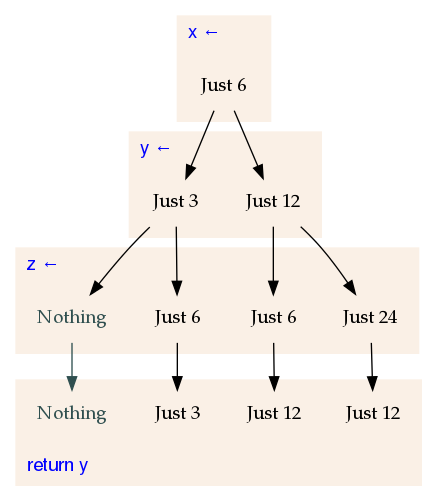
\includegraphics{/img/entries/list-monad/halvedouble.png}
\caption{\emph{halveOrDoubleDance 6}, all journeys illustrated}
\end{figure}

Huh. What happened here?

Again, there are four possible paths/journies\ldots{}only three of them end in success. In the
halve-halve path\ldots{}it fails. Now let's see what happens in the ``halve-double'' path. In this
case, it might be useful to look at the corresponding Maybe do-block, and using the choices we make
explicitly:

\begin{Shaded}
\begin{Highlighting}[]
\OtherTok{halveOrDoubleDance' ::} \DataTypeTok{Int} \OtherTok{->} \DataTypeTok{Maybe} \DataTypeTok{Int}
\NormalTok{halveOrDoubleDance' n }\FunctionTok{=} \KeywordTok{do}      \CommentTok{-- halveOrDoubleDance' 6}
    \NormalTok{x }\OtherTok{<-} \NormalTok{return n               }\CommentTok{-- Just 6}
    \NormalTok{y }\OtherTok{<-} \NormalTok{halve x                }\CommentTok{-- Just 3}
    \NormalTok{z }\OtherTok{<-} \NormalTok{double y               }\CommentTok{-- Just 6  (double n = Just n)}
    \NormalTok{return y                    }\CommentTok{-- Just 3}
\end{Highlighting}
\end{Shaded}

It is clear in this case that \texttt{return\ y} will give you the value of \texttt{y} \textbf{on
that path}.

In our halve-double path, the value of \texttt{y} (which is bound on the second line) is 3. That's
why when we say \texttt{return\ y}, it is \texttt{{[}3{]}}.

Remember --- you have to treat everything as its own individual path. In the halve-double path,
\texttt{y} is 3. So \texttt{return\ y} returns 3.

\subsection{Solving real-ish problems}\label{solving-real-ish-problems}

Okay, we are \emph{almost} ready to finally implement our solution to the Wolf/Goat/Cabbage puzzle.
Just one more demonstration.

Let's try this somewhat practical question:

``What operations on a number will make it a multiple of three?''

\begin{Shaded}
\begin{Highlighting}[]
\OtherTok{isMultThree ::} \DataTypeTok{Int} \OtherTok{->} \DataTypeTok{Bool}                              \CommentTok{-- 1}
\NormalTok{isMultThree a }\FunctionTok{=} \NormalTok{a }\OtherTok{`mod`} \DecValTok{3} \FunctionTok{==} \DecValTok{0}

\OtherTok{testNumber ::} \DataTypeTok{Int} \OtherTok{->} \NormalTok{[}\DataTypeTok{String}\NormalTok{]}
\NormalTok{testNumber n }\FunctionTok{=} \KeywordTok{do}
    \NormalTok{x }\OtherTok{<-} \NormalTok{return n                                       }\CommentTok{-- 2}
    \NormalTok{(f, fName)  }\OtherTok{<-}  \NormalTok{[ ((}\FunctionTok{*}\DecValTok{2}\NormalTok{)         , }\StringTok{"times two"}\NormalTok{)      }\CommentTok{-- 3}
                    \NormalTok{, ((}\FunctionTok{*}\DecValTok{3}\NormalTok{)         , }\StringTok{"times three"}\NormalTok{)}
                    \NormalTok{, ((}\FunctionTok{+}\DecValTok{2}\NormalTok{)         , }\StringTok{"plus two"}\NormalTok{)}
                    \NormalTok{, ((}\FunctionTok{+}\DecValTok{3}\NormalTok{)         , }\StringTok{"plus three"}\NormalTok{)}
                    \NormalTok{, ((}\FunctionTok{^}\DecValTok{2}\NormalTok{)         , }\StringTok{"square"}\NormalTok{)}
                    \NormalTok{, ((}\FunctionTok{+}\DecValTok{1}\NormalTok{)}\FunctionTok{.}\NormalTok{(}\FunctionTok{^}\DecValTok{2}\NormalTok{)    , }\StringTok{"square plus 1"}\NormalTok{)}
                    \NormalTok{, ((}\FunctionTok{+}\DecValTok{1}\NormalTok{)}\FunctionTok{.}\NormalTok{(}\FunctionTok{^}\DecValTok{3}\NormalTok{)    , }\StringTok{"cube plus 1"}\NormalTok{)}
                    \NormalTok{, (id           , }\StringTok{"stay the same"}\NormalTok{)}
                    \NormalTok{]}
    \KeywordTok{let} \NormalTok{z }\FunctionTok{=} \NormalTok{f x                                         }\CommentTok{-- 4}

    \NormalTok{guard }\FunctionTok{$} \NormalTok{isMultThree z                               }\CommentTok{-- 5}
    \NormalTok{return fName                                        }\CommentTok{-- 6}
\end{Highlighting}
\end{Shaded}

\begin{Shaded}
\begin{Highlighting}[]
\NormalTok{λ}\FunctionTok{:} \NormalTok{testNumber }\DecValTok{4}
\NormalTok{[}\StringTok{"times three"}\NormalTok{, }\StringTok{"plus two"}\NormalTok{]}
\NormalTok{λ}\FunctionTok{:} \NormalTok{testNumber }\DecValTok{5}
\NormalTok{[}\StringTok{"times three"}\NormalTok{, }\StringTok{"cube plus 1"}\NormalTok{]}
\NormalTok{λ}\FunctionTok{:} \NormalTok{testNumber }\DecValTok{6}
\NormalTok{[}\StringTok{"times two"}\NormalTok{, }\StringTok{"times three"}\NormalTok{, }\StringTok{"plus three"}\NormalTok{, }\StringTok{"square"}\NormalTok{, }\StringTok{"stay the same"}\NormalTok{]}
\NormalTok{λ}\FunctionTok{:} \NormalTok{testNumber }\DecValTok{7}
\NormalTok{[}\StringTok{"times three"}\NormalTok{, }\StringTok{"plus two"}\NormalTok{]}
\NormalTok{λ}\FunctionTok{:} \NormalTok{testNumber }\DecValTok{8}
\NormalTok{[}\StringTok{"times three"}\NormalTok{, }\StringTok{"cube plus 1"}\NormalTok{]}
\end{Highlighting}
\end{Shaded}

Let's go over this step-by-step:

\begin{enumerate}
\def\labelenumi{\arabic{enumi}.}
\tightlist
\item
  First of all, define the utility function \texttt{isMultThree\ a}, which is true when \texttt{a}
  is a multiple of three and false when it isn't.
\item
  In the block, \texttt{x} is set to be a choice in the journey. This choice is always going to be
  \texttt{n}, but if we wanted to test multiple numbers, we could do something like
  \texttt{x\ \textless{}-\ {[}n,\ n+1,\ n+2{]}}.
\item
  Now, the journey digerges. \texttt{f} and \texttt{fName} is now a value that depends on the path
  we took. If we took the first path, \texttt{f\ =\ (*2)} (the doubling function) and
  \texttt{fName\ =\ "times\ two"}. On the second path, \texttt{f\ =\ (*3)} (the tripling function)
  and \texttt{fName\ =\ "times\ three"}, etc.
\item
  We alias \texttt{z} to be the function we chose applied to \texttt{x}. If we had chosen the path
  \texttt{f\ =\ (*2)}, \texttt{z} would be \texttt{(*2)\ x}, which is \texttt{x*2}.
\item
  We check if \texttt{z} is a multiple of three. If it isn't, the journey sadly ends here. For
  example, if we called the function with \texttt{n\ =\ 4}, and we had chosen \texttt{f\ =\ (\^{}2)}
  (the square function), this journey (involving the choice of \texttt{(\^{}2)}) would meet its
  failure here\ldots{}but the journey with the choice \texttt{f\ =\ (+2)} would not!
\item
  At the end of the weary journey, we return the name of the function we chose. This step is never
  reached for failed journeys.
\end{enumerate}

Here is a diagram!

\begin{figure}[htbp]
\centering
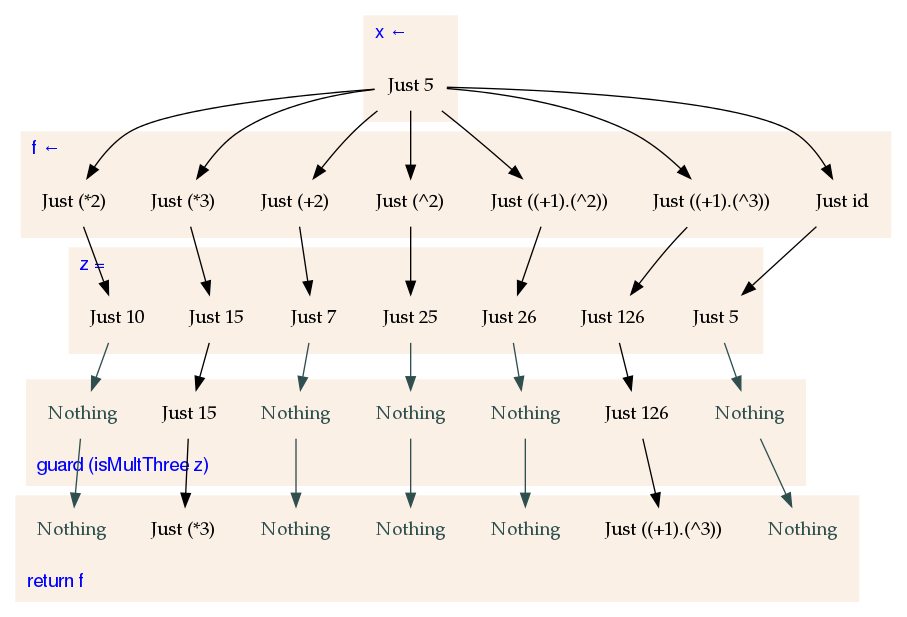
\includegraphics{/img/entries/list-monad/testnumber.png}
\caption{\emph{testNumber 5}, all journeys illustrated}
\end{figure}

\end{document}
